\documentclass{article}
\usepackage[utf8]{inputenc}
\usepackage{geometry}
\geometry{a4paper,left=2cm,right=2cm,top=1cm,bottom=1cm}
\title{Stat 605 Final Project Report}
\author{Yukun Fang, Mengkun Chen, Runze You, Mengqi Li}
\date{November 2020}
\usepackage{caption}
\usepackage{subfigure}
\usepackage{natbib}
\usepackage{graphicx}

\begin{document}

\maketitle

\section{Introduction}

In Sofia, air pollution norms were exceeded 70 times in the heating period from October 2017 to March 2018, citizens’ initiative AirBG.info says. During the time, the air pollution has become a serious problem for Sofia, This problem attracted the researchers all around the world.\\
\newline
Air Quality Index has been used to determine the level of air pollution across different regions worldwide. As part of it the levels of particulate matter (PM) is measured as well. This is the term used for a mixture of solid particles and liquid droplets found in the air. \\
\newline
Sofia air quality data set describes daily five air-quality measurements-PM2.5, PM10,  and climate statistics pressure, temperature
and humidity from July 2017 to June 2019.

\section{Analysis}


\subsection{\textbf{Data description}}
Our data sets are from 2017-7 to 2019-7 which contains every day of the two years. I take the head of two kind of dataset. We have make a \textbf{video} to show the change of PM10 and PM2.5 but here I use the plot to show the data for each month.
\begin{itemize}
    \item Pollution
    \begin{table}[ht]
    \centering
    \begin{tabular}{rrrrrrlrr}
    \hline
      & sensor\_id & location & lat & lon & timestamp & P1 & P2 \\ 
  \hline
1  & 2888 & 1453 & 42.71 & 23.28 & 2017-08-01T00:00:01 & 7.52 & 6.48 \\ 
  2  & 3641 & 1837 & 42.69 & 23.36 & 2017-08-01T00:00:02 & 10.70 & 6.10 \\ 
   \hline
\end{tabular}
\end{table}
\begin{figure}[ht]
	\centering
	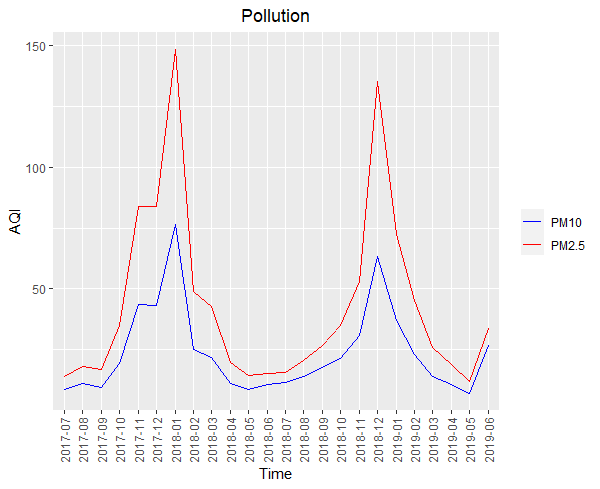
\includegraphics[width=8cm,height=6cm]{p1.png}
\end{figure}
sensor\_id: the id number of each sensor. There are 70-80 sensors for data sets.\\
lat: latitude\\
lon: longitude\\
P1: PM2.5\\
P2: PM10
    \item Climate
    \begin{table}[ht]
\centering
\begin{tabular}{rrrrrrlrr}
  \hline
  & sensor\_id & location & lat & lon & timestamp & pressure & temperature & humidity \\ 
  \hline
1  & 2266 & 1140 & 42.74 & 23.27 & 2017-07-01T00:00:07 & 95270.27 & 23.46 & 62.48 \\ 
  2  & 2292 & 1154 & 42.66 & 23.27 & 2017-07-01T00:00:08 & 94355.83 & 23.06 & 59.46 \\ 
   \hline
\end{tabular}
\end{table}
\begin{figure}[ht]
	\centering
	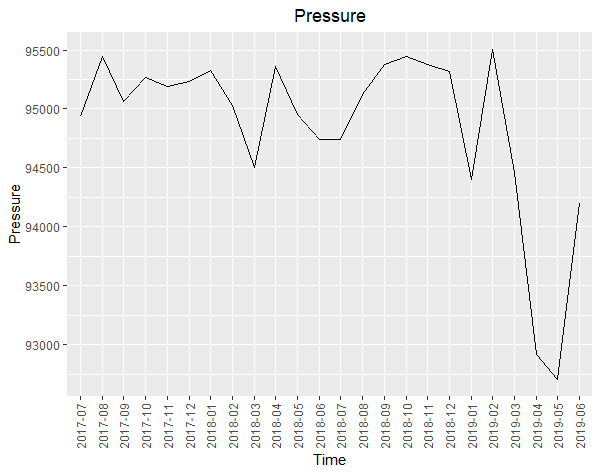
\includegraphics[width=6cm,height=4cm]{p2.png}
	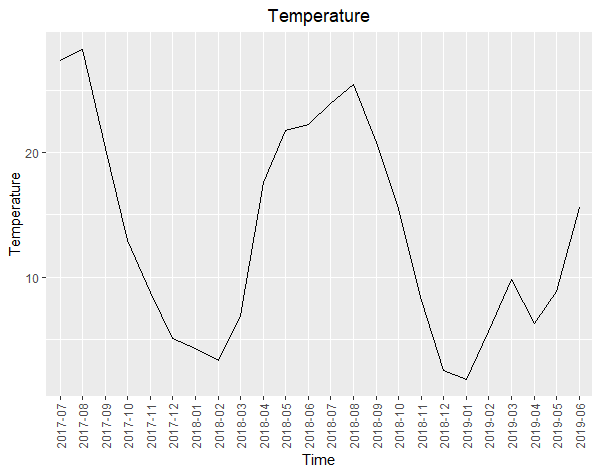
\includegraphics[width=6cm,height=4cm]{p3.png}
	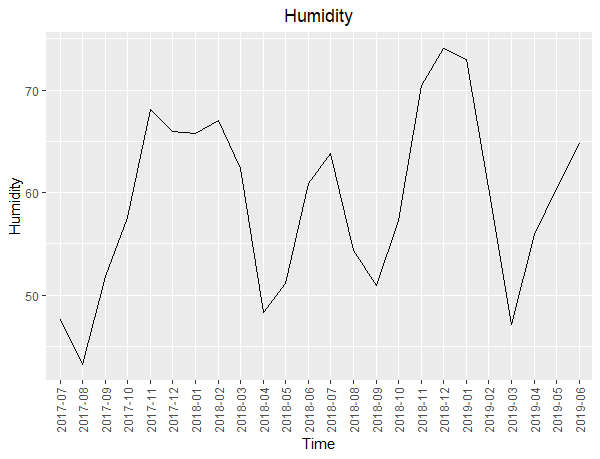
\includegraphics[width=6cm,height=4cm]{p4.png}
\end{figure}
\end{itemize}
\subsection{\textbf{Statistical analysis}}
According to the plots, we find that the pollution plot is a seasonal plot which contains two peaks in the winter month so we decide to test whether it is true.
\begin{figure}[ht]
	\centering
	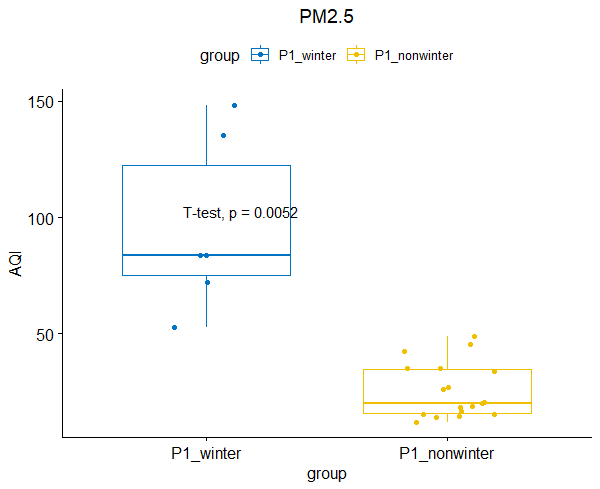
\includegraphics[width=8cm,height=6cm]{p5.png}
	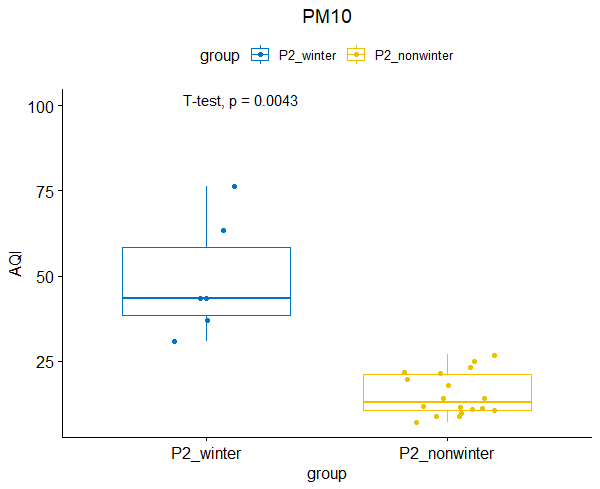
\includegraphics[width=8cm,height=6cm]{p6.png}
\end{figure}
According to the plot and the p-value, we can be sure that the winter is a time which the pollution is so heavy. To prove this, I draw the correlation plot to see their relationship.
\begin{figure}[ht]
	\centering
	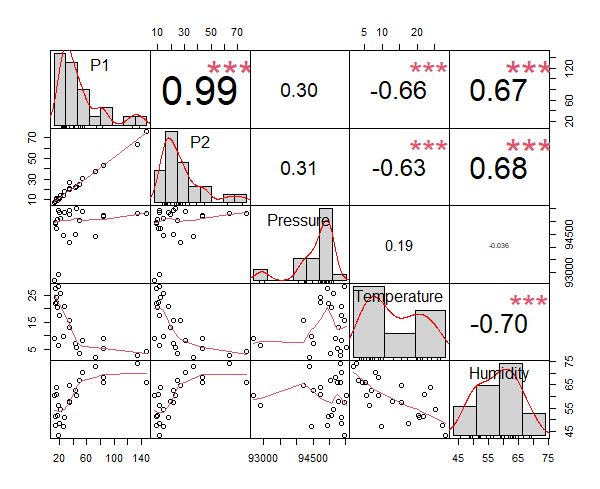
\includegraphics[width=7cm,height=6cm]{p7.png}
\end{figure}\\
Clearly PM1 and PM2 have great relationship with temperature and humidity.
\subsection{\textbf{Difficulties}}
It is difficult for us to show every day of two years. Actually we would make efforts to overcome that analyze every time in the data. Drawing pictures and run the code in CHTC cost a lot of time.

\section{Conclusion}
Sofia has a serious pollution problem which is especially in winter. It has relationship with temperature and humidity which git us a great signal to predict it. What we need to do in the future is to research the terrain of Sofia to make it more reasonable.


\end{document}
